\documentclass{article}
\usepackage[T1]{fontenc}
\usepackage[utf8]{inputenc}
\usepackage{lmodern}
\usepackage{amsmath}
\usepackage{sansmath}
\AtBeginDocument{\sansmath}
\renewcommand{\familydefault}{\sfdefault}
\usepackage[paperwidth=19cm,paperheight=14cm,margin=0.4cm]{geometry}
\usepackage{graphicx}
\usepackage{tikz}
\usetikzlibrary{positioning,fit,calc,arrows.meta,backgrounds,decorations.pathreplacing}
\pagestyle{empty}
\setlength{\parindent}{0pt}
\graphicspath{{img/}}

\definecolor{ink}{HTML}{0A0A0A}
\definecolor{muted}{HTML}{6A6A69}
\definecolor{line}{HTML}{BDBDBA}
\definecolor{red}{HTML}{E03A3A}
\definecolor{blue}{HTML}{2E6FE0}
\definecolor{yellow}{HTML}{D9A11A}
\definecolor{green}{HTML}{23A06A}
\definecolor{model}{HTML}{8C8C8A}

\tikzset{
  every picture/.style={font=\sffamily\small, line cap=round, line join=round},
  flecha/.style={-{Stealth[length=2.3mm,width=1.7mm]}, line width=0.7pt, draw=ink},
  grupo/.style={draw=#1, dash pattern=on 3pt off 2pt, line width=0.8pt, rounded corners=2pt, inner sep=6pt},
  titulo/.style={font=\sffamily\small\bfseries, text=#1, anchor=south west, inner sep=1pt},
  foto/.style={inner sep=0pt, outer sep=0pt, draw=ink, line width=0.5pt},
  caja/.style={draw=ink, line width=0.5pt, fill=#1, text=white, font=\sffamily\scriptsize\bfseries,
    text width=3.75cm, minimum height=0.46cm, align=center, inner sep=1.5pt},
  nota/.style={font=\sffamily\scriptsize, text=muted, align=center, inner sep=1pt},
  etapa/.style={font=\sffamily\footnotesize\bfseries, text=ink, align=center, inner sep=1pt},
  paso/.style={draw=ink, line width=0.5pt, fill=#1, text=ink, font=\sffamily\scriptsize, align=center,
    inner sep=3pt, minimum height=0.95cm, text width=2.35cm},
  paso/.default=white,
  grupofondo/.style={draw=#1, line width=0.8pt, fill=#1!6, rounded corners=3pt, inner sep=7pt},
  llave/.style={decorate, decoration={brace, mirror, amplitude=5pt, raise=2pt}, line width=0.7pt, draw=#1},
  llavetexto/.style={font=\sffamily\small\bfseries, text=#1, align=center},
}

\begin{document}
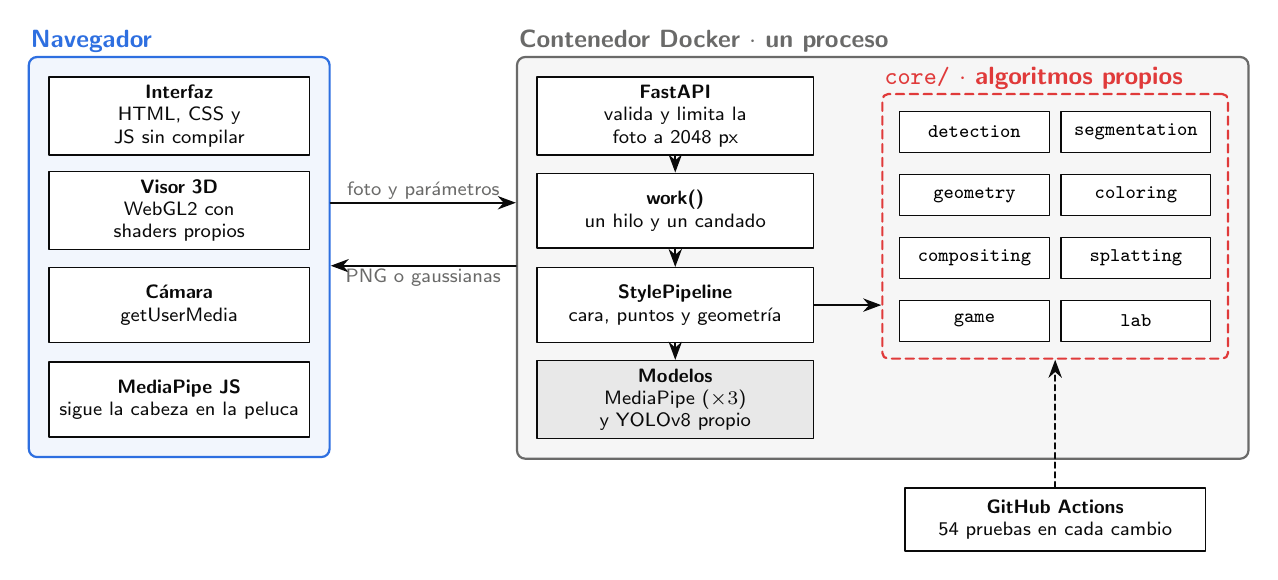
\begin{tikzpicture}

\foreach \name/\title/\text [count=\i] in {
  ui/Interfaz/{HTML, CSS y JS sin compilar},
  webgl/Visor 3D/{WebGL2 con shaders propios},
  cam/Cámara/{getUserMedia},
  mpjs/MediaPipe JS/{sigue la cabeza en la peluca}} {
  \node[paso, text width=3.1cm, minimum height=0.95cm] (b\name) at (0, {2.1 - 1.2 * (\i - 1)}) {\textbf{\title}\\\text};
}
\begin{scope}[on background layer]
  \node[grupofondo=blue, fit=(bui)(bmpjs)] (browser) {};
\end{scope}
\node[titulo=blue] at (browser.north west) {Navegador};

\node[paso, text width=3.3cm, minimum height=0.95cm] (api) at (6.3, 2.1) {\textbf{FastAPI}\\valida y limita la foto a 2048 px};
\node[paso, text width=3.3cm, minimum height=0.95cm] (work) at (6.3, 0.9) {\textbf{work()}\\un hilo y un candado};
\node[paso, text width=3.3cm, minimum height=0.95cm] (pipe) at (6.3, -0.3) {\textbf{StylePipeline}\\cara, puntos y geometría};
\node[paso=model!20, text width=3.3cm, minimum height=0.95cm] (models) at (6.3, -1.5) {\textbf{Modelos}\\MediaPipe ($\times3$) y YOLOv8 propio};

\foreach \name [count=\i from 0] in {detection, segmentation, geometry, coloring, compositing, splatting, game, lab} {
  \pgfmathsetmacro{\col}{mod(\i, 2)}
  \pgfmathsetmacro{\row}{int(\i / 2)}
  \node[draw=ink, line width=0.5pt, fill=white, font=\sffamily\scriptsize, minimum width=1.9cm, minimum height=0.52cm, inner sep=1pt]
    (m\i) at ({10.1 + 2.05 * \col}, {1.9 - 0.8 * \row}) {\texttt{\name}};
}
\node[grupo=red, fit=(m0)(m7)] (core) {};
\node[titulo=red] at (core.north west) {\texttt{core/} $\cdot$ algoritmos propios};

\begin{scope}[on background layer]
  \node[grupofondo=muted, fit=(api)(models)(core)] (docker) {};
\end{scope}
\node[titulo=muted] at (docker.north west) {Contenedor Docker $\cdot$ un proceso};

\draw[flecha] (browser.east |- 0, 1.0) -- node[above, nota] {foto y parámetros} (docker.west |- 0, 1.0);
\draw[flecha] (docker.west |- 0, 0.2) -- node[below, nota] {PNG o gaussianas} (browser.east |- 0, 0.2);
\draw[flecha] (api) -- (work);
\draw[flecha] (work) -- (pipe);
\draw[flecha] (pipe) -- (models);
\draw[flecha] (pipe.east) -- (core.west |- pipe.east);

\node[paso, text width=3.6cm, minimum height=0.8cm, anchor=north] (ci) at ($(core.south |- docker.south) + (0, -0.35)$) {\textbf{GitHub Actions}\\54 pruebas en cada cambio};
\draw[flecha, dash pattern=on 2pt off 1.5pt] (ci.north) -- (core.south);

\end{tikzpicture}
\end{document}
